\vspace{35mm}
\begin{figure}[h!]\centering
\captionsetup{width=\textwidth}
\caption{Average marginal electricity prices}
\label{fig:marg_price_5_default_rates}
\vspace{-2mm}
{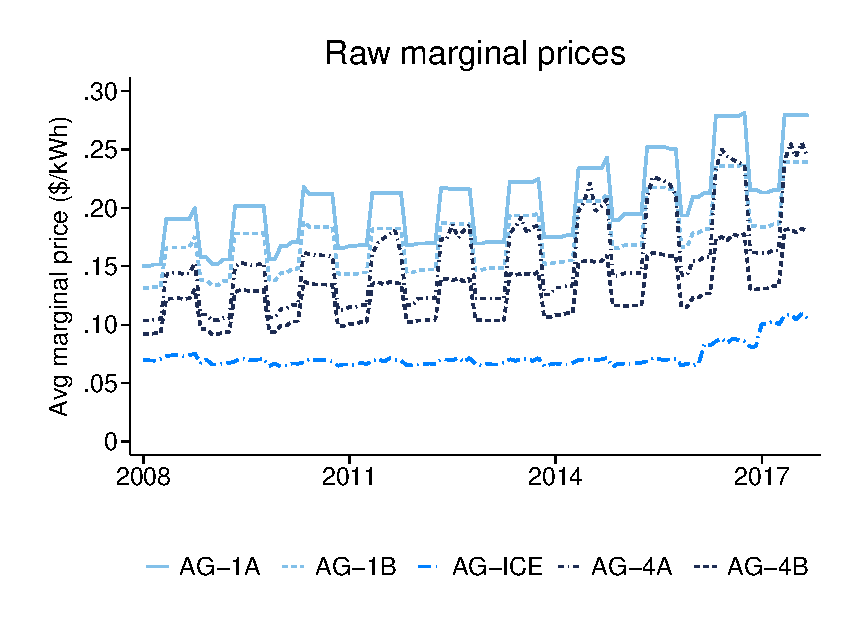
\includegraphics[width=.495\textwidth]{figures/marg_price_5_default_rates_raw.eps}}~
{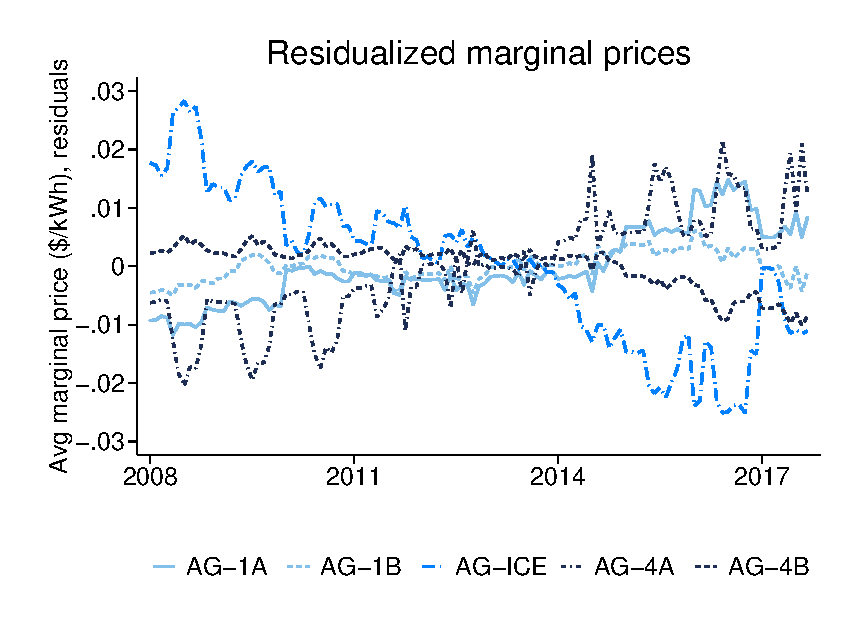
\includegraphics[width=.495\textwidth]{figures/marg_price_5_default_rates_resid.eps}}
\\
\captionsetup{width=\textwidth}
\caption*{\scriptsize \emph{Notes:} This figure plots times series of monthly average marginal electricity prices (\$/kWh) for PGE's five default agricultural tariffs. The left panel plots raw average marginal prices for each month in our estimation sample, taking unweighted averages across all hours. The right panel plots residuals of these same five time series, after partialing out tariff $\times$ month-of-year fixed effects and month-of-sample fixed effects (aligning with the fixed effects we use in estimation). AG-1A and AG-1B are non-time-varying rates (i.e.\ constant marginal price for all hours within a month), whereas AG-4A and AG-4B are time-varying rates (i.e.\ higher marginal prices during peak hours and weekdays). AG-1A and AG-4A are for small pumps ($<35$ hp), whereas AG-1B and AG-4B are for large pumps ($\ge35$ hp). AG-ICE is a time-varying rate for customers with auxiliary internal combustion engines. Marginal prices are systematically higher during summer months (May--October). Our identifying variation comes (a) strict restrictions that segment customers into categories; (b) the fact that the residualized default prices do not move in parallel; and (c) PGE's smart meter rollout, which exogenously shifted many customers from the AG-1A/1B default tariffs to the AG-4A/4B default tariffs with lower marginal prices.}
\end{figure}